% - - - - - - - - - - - - - - - - - - - - - - - - - - - - 
\subsection{PROCM-03 Registrar medicamento del proveedor}

\begin{figure}[htbp]
	\begin{center}
		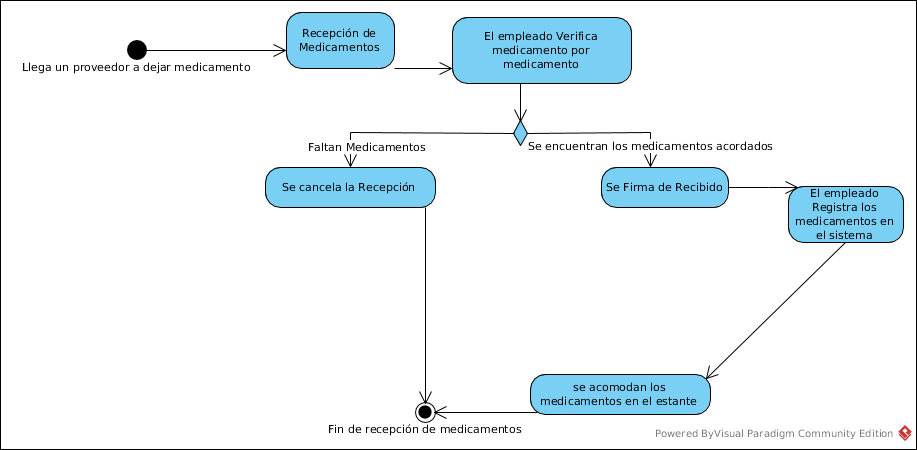
\includegraphics[width=.8\textwidth]{images/ToBEAgregarMedc}
		\caption{PROCM-03 Registrar medicamento del proveedor}
		\label{fig:proceso3}
	\end{center}
\end{figure}

\begin{description}
	\item[Descripción:] Cuando se llega un proveedor con un pedido de medicamento, 
	este se tiene que revisar y registrar en el sistema.
	\item[Entradas:] \cdtEmpty
        \begin{itemize}
			\item Datos del medicamento
        \end{itemize}
	\item[Salidas:] \cdtEmpty
        \begin{itemize}
			\item Dinero
        \end{itemize}	
    \item[Mejoras esperadas:] Este proceso es más lento que el anterior, pero ayuda a que existan menos incongruencias con los medicamentos en existencia, aparte de que ayuda a verificar de mejor forma los medicamentos que llegan del proveedor.
    \item[Casos de uso:] {CU 38 Registrar medicamentos del proveedor}, {CU 12 Listar medicamentos}.
\end{description}
